\chapter{Controlador de corriente} \chapterlabel{Informe/4-ControladorCorriente} \label{cap:ControladorCorriente}

En este capítulo se diseña y modela el circuito encargado de controlar la corriente que circula por el electroimán. Debido a que el sistema trabaja con corrientes elevadas se implementan estrategias de conmutación con el fin de reducir las pérdidas de energía. Para ello se utiliza una topología de puente H con cuatro MOSFET y un \textsl{bootstrap driver} que los controla. Además, se detallan los criterios tenidos en cuenta al momento de  elegir  y dimensionar todos los componentes que intervienen para lograr el correcto funcionamiento del controlador de corriente. Por último, se obtiene su función transferencia  para ser utilizada en el diseño del compensador.

\section{Descripción general}

\noindent Para regular la fuerza ejercida por el electroimán es necesario controlar la corriente que circula por él. Para ello, se modela a la planta como la admitancia de un circuito RL serie, cuya inductancia varía con el entrehierro como se observa en la expresión \ref{eq_admitancia}.

\begin{equation} \label{eq_admitancia}
\frac{1}{sL(Y_g)\ +\ R_L}
\end{equation}

\noindent Para realizar este control se utiliza un sistema realimentado, como el que se muestra en la figura \ref{fig:img_diag-en-bloques}. La entrada al sistema es una tensión de referencia ($V_{iLRef}$) proporcional a la corriente de salida deseada, que luego se multiplica por la ganancia de entrada ($K_{in}$). La corriente del electroimán se realimenta en forma de una tensión proporcional a ella ($V_{iLF}$). Ambas tensiones son restadas y el resultado ($V_e$) ingresa al bloque del comparador con histéresis, que actúa en conmutación, por lo que su salida tiene dos estados posibles: $\pm$$V_L$.

\noindent Al ser aplicadas al inductor se produce una rampa de corriente: si la tensión es positiva, la rampa crece, y si es negativa decrece. De esta forma, debido a la conmutación del comparador se obtiene, a la salida, una forma de onda triangular $I_L$, cuyo valor medio es la corriente deseada y es proporcional a la tensión de referencia.

\begin{figure}[H]
	\centering
	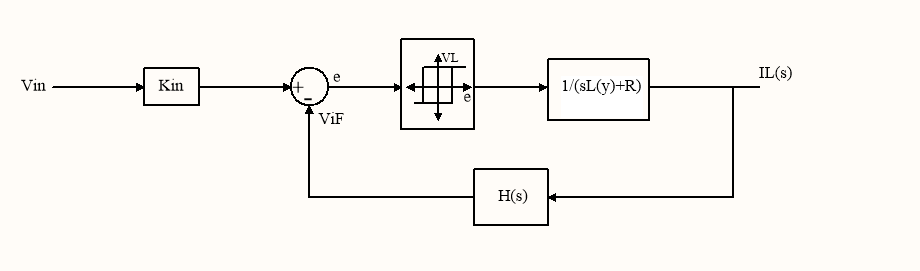
\includegraphics[width=\textwidth]{Diagrama-en-bloques.png}
	\caption{Diagrama en bloques simplificado del controlador de corriente.}
	\label{fig:img_diag-en-bloques}
\end{figure}

\section{Circuito del controlador de corriente}

\noindent Se plantea la etapa de entrada que consiste en la ganancia $K_{in}$ y el restador con la señal realimentada. El objetivo es que una tensión de referencia en la entrada entre $0\:V$ y $5\:V$ se corresponda de manera lineal con una corriente de salida entre $0\:A$ y $30\:A$ (en valor medio). Por lo tanto, se obtiene una ganancia del controlador de corriente de $6\:A/V$. Para sensar la corriente se eligió utilizar un sensor de efecto Hall HO 15-NP \cite{HO15-NP} cuya transconductancia es de $H(s) = 53.3\:mV/A$. De esta manera la ganancia de entrada se calcula como:

\begin{equation}
	K_{in}=\frac{30\:A*53.3\:mV/A}{5\:V}=0.32 
\end{equation}


La salida de esta etapa, al igual que la tensión de salida del sensor de efecto Hall, se polarizan en un punto de operación de $2.6\:V$ (ver sección \ref{secc_justificación-puente-H}). Para lograrlo se utiliza un circuito como el que se muestra en la figura \ref{fig:img_etapa-de-entrada}.


\begin{figure}[H]
	\centering
	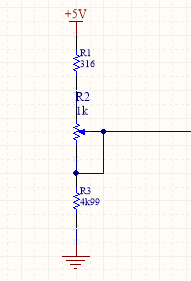
\includegraphics[scale=1]{Etapa-de-entrada.png}
	\caption{Etapa de entrada.}
	\label{fig:img_etapa-de-entrada}
\end{figure}

Para la implementación del comparador con histéresis se utiliza un amplificador operacional realimentado positivamente. Se eligió que la corriente de salida del electroimán tenga un ripple de $500\:mA$. Por lo tanto, al afectar este valor por la transconductancia del sensor de efecto Hall, se obtiene un ancho de histéresis de $26.665\:mV$, alrededor de un punto de operación de $2.5\:V$. El circuito implementado se muestra en la figura \ref{fig:img_comp-con-hist}.

\begin{figure}[H]
	\centering
	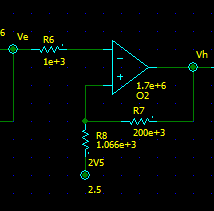
\includegraphics[scale=1]{Comparador-con-histeresis.png}
	\caption{Comparador con histéresis.}
	\label{fig:img_comp-con-hist}
\end{figure}

Para controlar la corriente se utiliza un \textsl{driver} que trabaja en conmutación con una topología en puente H con cuatro N-MOS. Este permite conmutar la polaridad de la tensión aplicada al electroimán entre $+24\:V$ para el estado ON y $-24\:V$ para el OFF. 

Para poder realizar simulaciones se modela al sensor de efecto Hall como una fuente de tensión controlada por corriente con una ganancia de $53.3\:mV/A$, cuya salida es realimentada a la etapa de entrada luego de restarle la tensión de referencia  $V_{bias}$ de $2.5\:V$, como se muestra en la figura \ref{fig:img_resta-Vbias}.

La implementación circuital de estas dos etapas puede observarse en la figura \ref{fig:img_puenteH}. 


\begin{figure}[H]
	\centering
	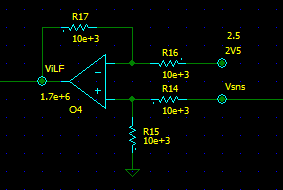
\includegraphics[scale=1]{Resta-Vbias.png}
	\caption{Resta de $V_{bias}$ al sensor de efecto Hall.}
	\label{fig:img_resta-Vbias}
\end{figure}

\begin{figure}[H]
	\centering
	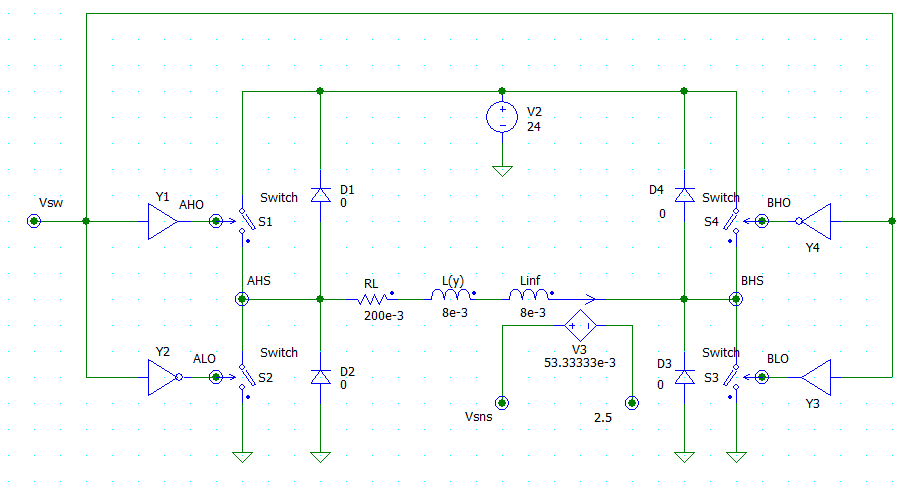
\includegraphics[scale=0.8]{PuenteH.png}
	\caption{Puente H y sensor de efecto Hall.}
	\label{fig:img_puenteH}
\end{figure}

\subsection{Simulaciones de formas de onda}

\noindent En la figura \ref{fig:img_formas-de-onda-corriente} se pueden observar dos formas de onda. La inferior  corresponde a la tensión de salida del comparador con histéresis y la superior a la corriente que circula por el electroimán. Para la simulación se utilizó una tensión de referencia de entrada de $1\:V$, por lo que el valor medio de la corriente en la salida es $6\:A$ con un ripple de $500\:mA$.

\begin{figure}[H]
	\centering
	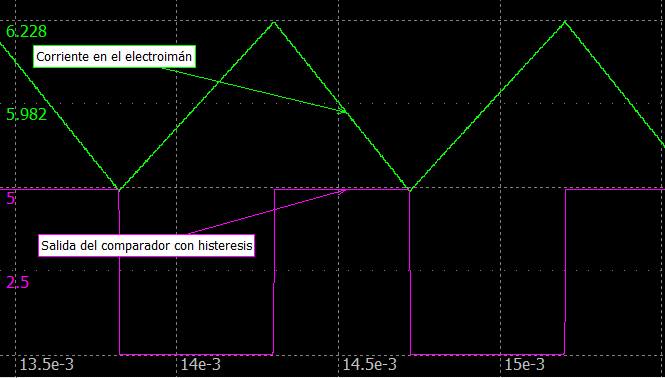
\includegraphics[scale=0.5]{Formas-de-onda-corriente.png}
	\caption{Formas de onda de corriente en el electroimán y tensión de salida del comparador.}
	\label{fig:img_formas-de-onda-corriente}
\end{figure}



\subsection{Simulación de un escalón en la referencia de corriente}

\noindent En la figura \ref{fig:img_respuesta-al-escalon} se muestra cómo cambia la corriente en el electroimán al aplicarle a la entrada del controlador un escalón de tensión entre $1\:V$ y $3\:V$. Se puede observar cómo la conmutación del comparador se detiene para ajustar la corriente con la referencia.

\begin{figure}[H]
	\centering
	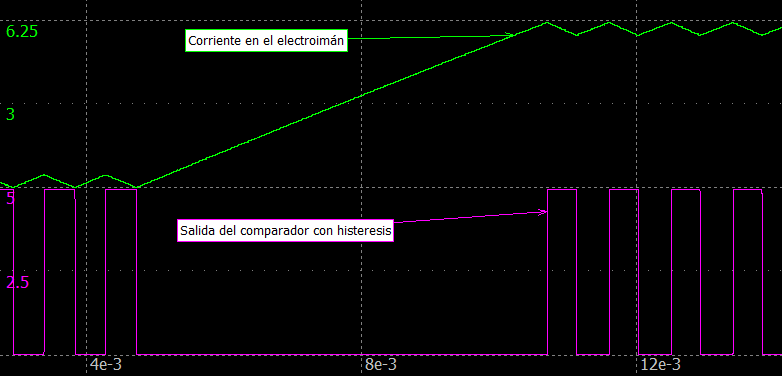
\includegraphics[scale=0.5]{Respuesta-al-escalon.png}
	\caption{Respuesta al escalón del circuito.}
	\label{fig:img_respuesta-al-escalon}
\end{figure}


\subsection{Descripción general de la topología}

\noindent Se desea controlar la corriente que circula por el electroimán y, debido a que el sistema va a trabajar con corrientes elevadas, es importante que la implementación del controlador de corriente sea eficiente. Por lo tanto, para disminuir la disipación de potencia del circuito se utiliza un controlador que funciona en conmutación. 

\noindent Para lograr una corriente contínua en el electroimán mediante una fuente conmutada se debe alternar la polaridad de la tensión aplicada en los bornes del inductor. De esta forma, la corriente crece y decrece (según la polaridad) con forma exponencial debido a la resistencia interna del electroimán. Sin embargo, como el intervalo de tiempo de esta conmutación es pequeño comparado con la constante de tiempo de la planta, el incremento de corriente será pequeño y puede ser aproximado a una recta. Por lo tanto, se obtiene una corriente contínua con un ripple superpuesto de forma triangular. 

\noindent Para lograr alternar la polaridad de la fuente sobre el inductor se utiliza una topología en puente H con cuatro MOSFET manejados por el controlador por histéresis como se observa en la figura \ref{fig:img_topologia-puenteH}. Pueden diferenciarse dos semiciclos de trabajo: uno de estado ON y otro de estado OFF. El primero se define como el semiciclo durante el cual la corriente en el inductor crece (pendiente positiva), mientras que el segundo se da cuando la corriente decrece.

\begin{figure}[H]
	\centering
	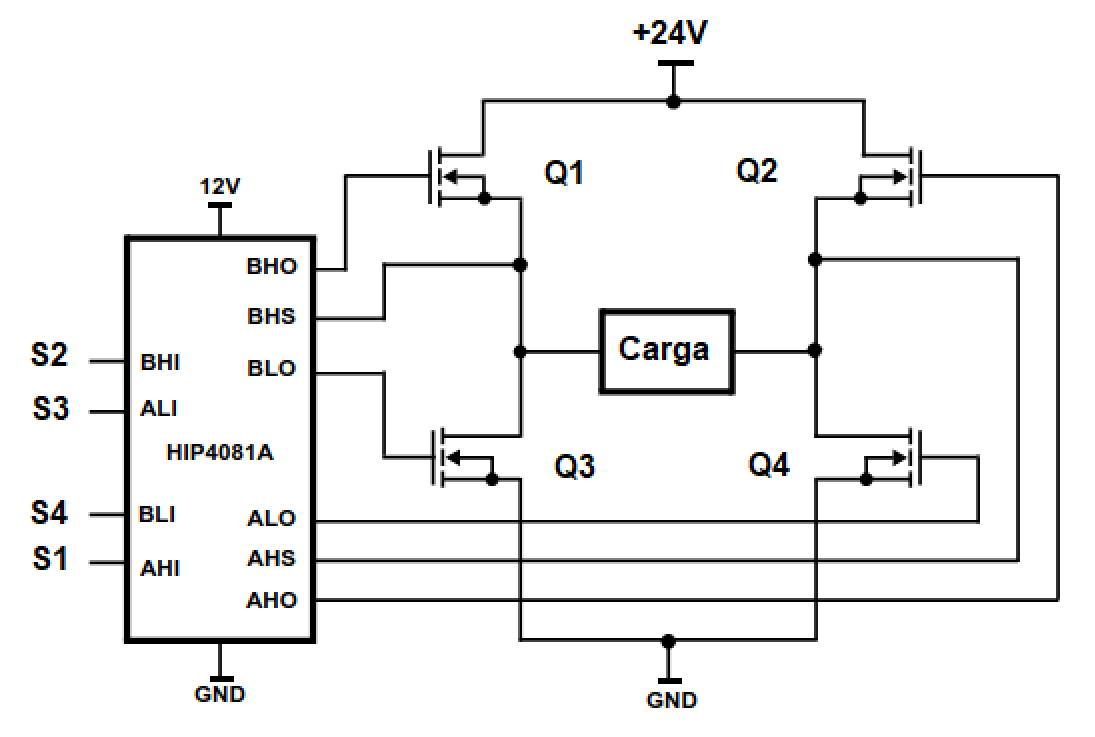
\includegraphics[scale=0.7]{Topologia-puenteH.png}
	\caption{Topología elemental del puente H.}
	\label{fig:img_topologia-puenteH}
\end{figure}

\noindent El electroimán se conecta entre los puntos medios de cada par de transistores. De esta manera se puede conmutar la polaridad de la tensión que se le aplica. Sólo se permite que dos transistores se enciendan a la vez, y esto se realiza de manera diagonal. Es decir, en la figura \ref{fig:img_topologia-puenteH}, $Q_1$ y $Q_4$ pueden estar encendidos, mientras que $Q_3$ y $Q_2$ están apagados, y viceversa. De otra forma, se podría generar un cortocircuito entre la fuente de alimentación y GND, que produciría una circulación de corriente denominada \textsl{shoot-through}. 


\noindent Los cuatro MOSFET utilizados para el puente H son de tipo N. Para que estos puedan funcionar correctamente en conmutación es necesario que en el estado ON, la diferencia de tensión entre \textsl{gate} y \textsl{source} sea mayor o igual a $7\:V$. Esto no es un problema para los dos MOS inferiores del puente H ($Q_2$ y $Q_4$), ya que la tensión en \textsl{source} está fijada en GND y el \textsl{driver} puede aplicar $12\:V$ al \textsl{gate} (superando los $7\:V$ entre \textsl{gate} y \textsl{source}). El problema radica en los transistores superiores del puente H, ya que la tensión en \textsl{source} varía entre $0\:V$ y $24\:V$, por lo que en el \textsl{gate} debería haber, por lo menos, $31\:V$ con respecto a GND. Sin embargo, la tensión máxima disponible entregada por la fuente es de $24\:V$. Para resolver este problema se utiliza un \textsl{driver} flotante con \textsl{bootstrap}.

\noindent Para controlar la conmutación se utiliza un MOSFET \textsl{driver} HIP4081A \cite{HIP4081A_FN3659} que se encarga de encender y apagar los transistores según las entradas de control. Además permite la configuración de un tiempo muerto para evitar que se enciendan dos transistores de un lado a la vez. También provee la circuitería necesaria para implementar la fuente flotante que enciende los MOSFET del lado superior para lo cual solo se debe agregar un diodo y un capacitor de manera externa. Para la implementación circuital se van a utilizar los MOSFET IPB160N04 \cite{IPB160N04}.

\noindent En la figura \ref{fig:img_bootstrap} se observa solo una de las mitades del puente H (lado A)  junto con las señales de control provistas por el \textsl{driver} HIP4081A. El análisis para la otra mitad es análogo, por lo que se evita por simplicidad. La implementación del \textsl{bootstrap driver} permite obtener en el \textsl{gate} del MOS superior, una tensión de $36\:V$ respecto a GND, de manera que se logra una diferencia de tensión mayor a $7\:V$ entre \textsl{gate} y \textsl{source}. 

\begin{figure}[H]
	\centering
	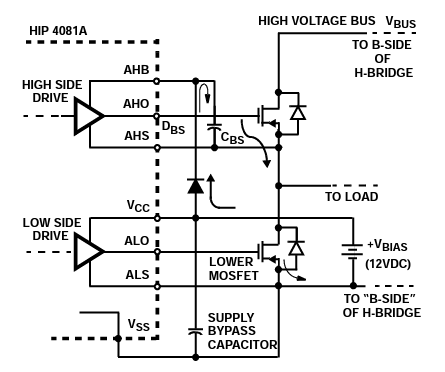
\includegraphics[scale=0.7]{Bootstrap.png}
	\caption{Configuración \textsl{bootstrap} simplificada.}
	\label{fig:img_bootstrap}
\end{figure}

\noindent El \textsl{bootstrap driver} consiste en un capacitor ($C_{BS}$), un diodo, y la circuitería interna del HIP4081A. Para garantizar el correcto funcionamiento del \textsl{bootstrap}, al encender el sistema, la secuencia de inicio del HIP4081A enciende las dos salidas de la parte inferior del puente H: ALO y BLO con el fin de encender $Q_2$ y $Q_4$ durante un tiempo que se conoce como periodo de refresco de \textsl{bootstrap}. De esta forma, los capacitores de \textsl{bootstrap} de ambos lados quedan conectados entre $12\:V$ y GND y se pueden cargar completamente. Durante este tiempo, las salidas a los \textsl{gates} AHO y BHO se mantienen en bajo continuamente lo que asegura que no se produzca corriente de \textsl{shoot-through} durante el período nominal de refresco del \textsl{bootstrap}. Una vez finalizado, las salidas responden normalmente al estado de las señales de entrada de control.

\noindent Para comprender su funcionamiento se hará un breve análisis del sistema. Para ello, se parte de la suposición de que el sistema se encuentra en funcionamiento: con el transistor $Q_2$ encendido (ALO = $V_{CC}$), $Q_1$ apagado (AHO = AHS = $0\:V$) y la corriente circulando de izquierda a derecha como lo indica la figura \ref{fig:img_bootstrap}. En ese caso, el capacitor $C_{BS}$ se carga a $12\:V$, ya que en un terminal tiene la fuente de $12\:V$ (a través del diodo $D_{BS}$) y el otro está conectado a GND por medio de $Q_2$.

\noindent Una vez que se apaga el transistor inferior, empieza a transcurrir el tiempo muerto. Debido a que la carga es inductiva, el valor medio de la corriente mantiene su sentido y circula por los diodos antiparalelos del MOS inferior del lado A y el superior del lado B. Esto provoca que el \textsl{source} del MOS superior del lado A tenga una tensión negativa igual a la caída de tensión en directa del diodo antiparalelo de $Q_2$. 

\noindent Una vez finalizado el tiempo muerto, se enciende el MOS $Q_1$. Para ello, la señal AHO se pone en nivel alto. Durante el tiempo que $Q_1$ pasa de estar apagado a encendido, la tensión en el \textsl{source} cambia de $-V_d$ a $V_{bus}$ de manera gradual mientras se carga el \textsl{gate}, y AHO pasa a ser igual a AHB, que es igual a la tensión entregada por el capacitor de \textsl{bootstrap} sumada a la tensión en el \textsl{source} de $Q_1$. De esta manera se logra una tensión de $36\:V$ con respecto a GND en el \textsl{gate} y genera una diferencia entre \textsl{gate} y \textsl{source} de $12\:V$.

\noindent Para lograr un funcionamiento adecuado del \textsl{bootstrap} es necesario dimensionar correctamente al capacitor $C_{BS}$ con el fin de que pueda proveer la carga suficiente durante el tiempo en el que el MOS esté encendido.


\subsection{Dimensionamiento de capacitor de \textsl{bootstrap}}

\noindent Para el dimensionamiento de los capacitores de \textsl{bootstrap} se tuvieron en cuenta sugerencias y procedimientos descriptos en \cite{HIP4081A_AN9405} y \cite{HIP4081A_FN3659}.

\noindent Para encender un NMOS es necesario proveer corriente a su \textsl{gate} hasta cargar las capacidades parásitas entre \textsl{gate-source} y \textsl{gate-drain}. Una vez cargadas, el MOS queda en estado encendido y no consume más corriente en el \textsl{gate}. En el caso de los MOS del lado superior, esta corriente proviene del capacitor de \textsl{bootstrap}. 

\noindent En la implementación del puente H se decidió colocar resistencias entre \textsl{gate} y \textsl{source} (ver apartado \ref{secc_res_gate_source}), que aparecen como $R_1$, $R_2$, $R_3$ y $R_4$ en la figura \ref{fig:img_capacitores-puenteH}. Debido a la diferencia de tensión entre \textsl{gate-source}, se genera una corriente constante en estas resistencias durante el tiempo que el MOS esté encendido, que también debe ser provista por el  \textsl{bootstrap}.

\begin{figure}[H]
	\centering
	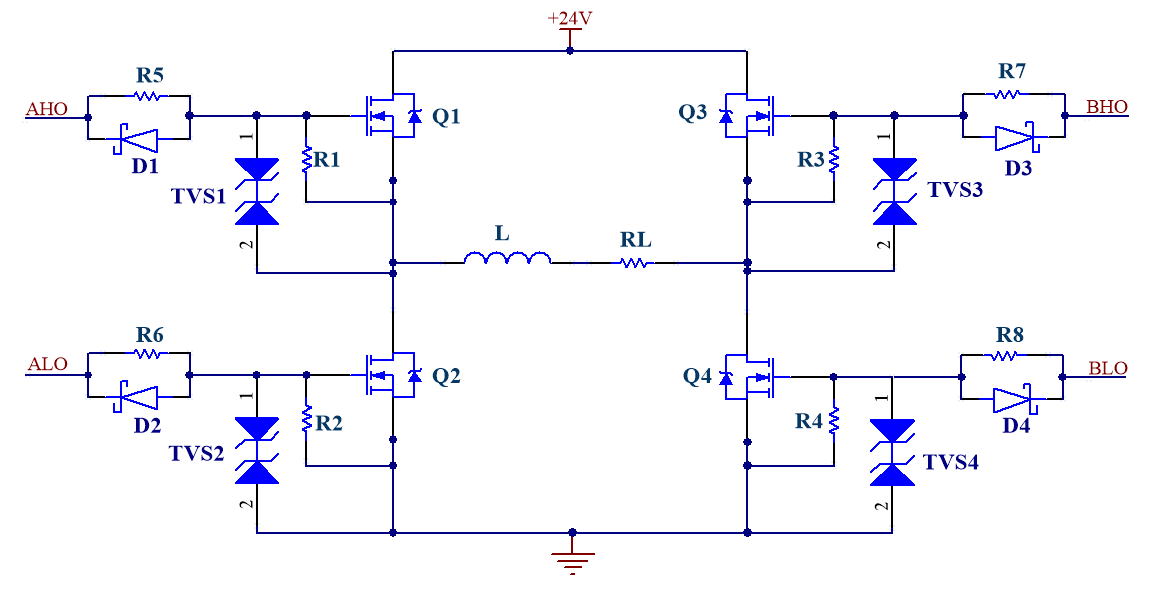
\includegraphics[scale=0.6]{Capacitores-puenteH.png}
	\caption{Puente H.}
	\label{fig:img_capacitores-puenteH}
\end{figure}

\noindent Por otro lado, el capacitor debe entregar corriente al diodo de \textsl{bootstrap} cuando este queda en inversa ($I_{DR}$), y también entregar una corriente de fuga al circuito integrado HIP ($I_{QBS}$). Esta última se desprecia ya que es compensada internamente por la bomba de carga del HIP.

\noindent Por lo tanto, para poder dimensionar correctamente el capacitor de \textsl{bootstrap} es necesario tener en cuenta todos los efectos mencionados anteriormente. Para ello se parte planteando la carga que almacena el capacitor \textsl{bootstrap}:

\begin{equation} \label{eq_carga-cap-bootstrap}
Q_{BS}=C_{BS}*\Delta V_{BS}
\end{equation}

\noindent En la ecuación \ref{eq_carga-cap-bootstrap}, $Q_{BS}$ es la carga total del capacitor de \textsl{bootstrap}, $C_{BS}$ su capacidad, y $\Delta V_{BS}$ es la diferencia de  tensión entre sus terminales. 

\noindent Para evitar sufrir una caída de tensión tal que afecte el encendido de los MOS, es necesario que $Q_{BS}$ pueda abastecer también al \textsl{gate}, al diodo en inversa y a la resistencia entre \textsl{gate-source}. Por lo tanto:

\begin{equation} \label{eq_carga-cap-bootstrap2}
Q_{BS} > Q_G + Q_{RR} + \frac{I_{DR}+I_{GS}}{f_{PWM}}
\end{equation}

\noindent Donde:
\begin{itemize}
\item $Q_G$ = Carga total que se debe entregar al \textsl{gate} del MOS.
\item $Q_{RR}$ = Carga entregada al diodo en inversa durante el tiempo de recuperación (cuando pasa de modo conducción a inversa).
\item $I_{DR}$ = Corriente de fuga del diodo en inversa.
\item $I_{GS}$ = Corriente que circula por la resistencia de \textsl{gate-source}.
\item $f_{PWM}$ = frecuencia de conmutación.
\end{itemize}


\noindent Por lo tanto, al reemplazar la ecuación \ref{eq_carga-cap-bootstrap} en la \ref{eq_carga-cap-bootstrap2} resulta:


\begin{equation} \label{eq_cap-bootstrap}
C_{BS} > \frac{Q_G+Q_{RR} + \frac{I_{DR}+I_{GS}}{f_{PWM}}}{\Delta V_{BS}}
\end{equation}

\noindent Según la hoja de datos \cite{IPB160N04} del MOSFET IPB160N04, se obtiene que $Q_G= 170\:nC$. Por lo tanto, al adoptar una caída de tensión tolerable en el capacitor de $\Delta V_{BS} = 0.1\:V$, es posible dimensionarlo para que posea carga suficiente para mantener al MOSFET siempre encendido.

\noindent Para el cálculo de la carga de recuperación $Q_{RR}$ se puede considerar que la forma de onda de la corriente de recuperación es triangular. De esta forma,  $Q_{RR}$ es aproximadamente igual a la mitad del producto entre el pico de la magnitud de corriente inversa y la duración del tiempo de recuperación.  Debido a que se usa el diodo RSX205LAM30TR se obtiene, a partir de \cite{RSX205LAM30}, que  $I_R$ es igual a $0.1\:A$  y  el tiempo de recuperación de inversión es de $12.5\:ns$. Por lo tanto, la carga de recuperación resulta de $0.625\:nC$. Además, la corriente inversa de fuga del diodo de \textsl{bootstrap} tiene un valor de $I_{DR} =2 \:mA\:(@\: T=75^{\circ}\:C, V_R= 24\:V)$.

\noindent La corriente $I_{GS}$ tiene forma exponencial pero se aproxima a una constante debido a que el intervalo de tiempo es pequeño. Por lo tanto, puede calcularse como la diferencia de tensión del capacitor de \textsl{bootstrap} ($V_B=12\:V$) dividido el valor de la resistencia \textsl{gate-source}, que es de $4.7\:k\Omega$. Por lo tanto, $I_{GS}=2.55 \:mA$. 

\noindent Debido a que el controlador por histéresis no asegura que haya una conmutación en un tiempo constante (como se observa en la figura \ref{fig:img_respuesta-al-escalon}), se decidió superponer una conmutación auxiliar de $50\:kHz$ (como se explica en el apartado \ref{secc_conmutacion-auxiliar}), lo que resulta en $f_{PWM}=50 \:kHz$. 

\noindent Al reemplazar los valores obtenidos en \ref{eq_cap-bootstrap}, se obtiene:

\begin{equation} 
	\begin{aligned}
		C_{BS} &> \frac{170 \:nC + 0.625\:nC + \frac{2 \:mA + 2.55 \:mA}{50 \:kHz}}{0.1 \:V}\\
	\end{aligned}
\end{equation}

\begin{equation} 
	\begin{aligned}
		C_{BS} &> 2.61 \:\mu F\\	
	\end{aligned}
\end{equation}


\noindent Por lo tanto, una capacidad mayor a $2.61 \:\mu F$ resulta en una caída menor a $0.1\:V$ en el capacitor de \textsl{bootstrap} durante el tiempo de encendido de los MOSFET. Podría usarse un capacitor más pequeño, a costa de permitir una mayor caída de tensión en el capacitor. 

\noindent Finalmente, se decidió utilizar dos capacitores de \textsl{bootstrap} en paralelo de $5.6 \:\mu F$ cada uno, con el objetivo de reducir la resistencia serie.


\subsection{Resistencia entre \textsl{gate} y \textsl{source}} \label{secc_res_gate_source}

\noindent Se colocan resistencias que conectan el \textsl{gate} y el \textsl{source} de cada MOS en el puente H. Estas se observan en la figura \ref{fig:img_capacitores-puenteH} como $R_1$, $R_2$, $R_3$ y $R_4$. Su propósito es evitar que el \textsl{gate} del MOSFET se encuentre cargado cuando el circuito se enciende y el \textsl{driver} de corriente aún no puede descargarlo. Además, ayuda a evitar que se encienda el MOSFET por ruido acoplado capacitivamente. 

\noindent Se utiliza una resistencia de $4.7 \:k\Omega$ debido a que permite que el \textsl{gate} se descargue en un tiempo rápido, consumiendo solo $2.55\:mA$ del capacitor de \textsl{bootstrap}.

\subsection{Protección del \textsl{gate}}

\noindent El \textsl{gate} de los MOS es sensible a las sobretensiones. Soporta como máximo $\pm 20\:V$. Una descarga electrostática (ESD) puede sobrepasar ampliamente este valor de tensión y dañar el MOS al acercar la mano o la sonda del osciloscopio. Para protegerlo se coloca un diodo TVS entre el \textsl{gate} y \textsl{source} de cada transistor, de manera de limitar la tensión que se desarrolla en el \textsl{gate} a un valor seguro.

\noindent Se eligen los TVS SMAJ15 con una tensión bidireccional de $\pm 15\:V$.

\subsection{Tiempo muerto}

\noindent Para evitar generar un cortocircuito durante la conmutación de los transistores, el \textsl{driver} HIP4081A permite configurar un tiempo muerto que debe transcurrir desde que se apaga un transistor y se enciende el próximo. Esto se configura mediante dos resistencias conectadas a sus pines LDEL y HDEL.

\noindent Para saber el tiempo muerto necesario, debe conocerse el tiempo que tarda en apagarse un MOSFET IPB160N04. De \cite{IPB160N04} se obtiene que este tiempo es de $63\:ns$ (teniendo en cuenta el $T_{OFF}$ y el $T_{FALL}$). Por lo tanto, al considerar que esta aplicación espcífica no requiere un tiempo de encendido rápido de los MOSFET, se elige que el tiempo muerto sea de $100\:ns$.

\noindent Según la hoja de datos del HIP4081A, para obtener ese tiempo muerto, las resistencias en HDEL y LDEL deben ser $200\:k\Omega$.

\subsection{Dimensionamiento de los capacitores de fuente}
	
\noindent Para reducir el consumo de potencia de la red se utilizan capacitores en paralelo a la fuente de $+24\:V$. Esto permite que, una vez que la fuente cargó inicialmente el inductor, en las conmutaciones sucesivas la carga del inductor pase a dichos capacitores en un semiciclo y viceversa en el otro ciclo de conmutación. Idealmente, esta transferencia de energía no tiene pérdidas. Por lo tanto, el consumo de potencia queda reducido a la perdida por disipación de los MOSFET y los demás componentes del controlador de corriente. 

\noindent Estos capacitores deben tener una baja resistencia equivalente serie (ESR) ya que, de lo contrario, disiparían mucha potencia en forma de calor y se acortaría su vida útil. Además generan ripple en la tensión $V_{BUS}$.

\noindent En la figura \ref{fig:img_capacitores-puenteH} los capacitores de la fuente están representados por $C_1$ y $C_2$. Para poder dimensionarlos correctamente hay que tener en cuenta que la forma de onda de la corriente que circula por el electroimán en régimen permanente es aproximadamente triangular. Esta corriente es conducida durante medio ciclo desde estos capacitores hacia el electroimán por $Q_1$ y $Q_4$. Luego, durante la otra mitad del ciclo, la corriente regresa a estos capacitores a través de $Q_2$ y $Q_3$. Esto provoca que la corriente en los capacitores sea, durante el semiciclo encendido, igual al valor medio de la corriente del electroimán, con $ \pm \frac{\Delta I_L}{2}$. Similarmente ocurre en el semiciclo apagado, pero con valor medio $-<I_L>$.  Por lo tanto,  la corriente tiene la forma que se muestra en la figura \ref{fig:img_ccorriente-capacitores}

\begin{figure}[H]
	\centering
	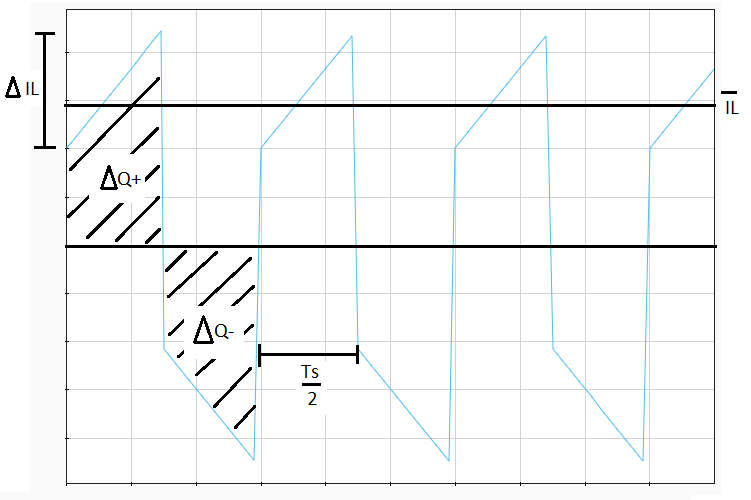
\includegraphics[scale=0.6]{Corriente-capacitores.png}
	\caption{Forma de onda de la corriente en $C_1$ y $C_2$.}
	\label{fig:img_ccorriente-capacitores}
\end{figure}

\noindent Por el electroimán circula una corriente media de aproximadamente $21\:A$ en condiciones normales de trabajo. Por lo tanto, la carga del capacitor se puede calcular como:

\begin{equation} 
	\begin{aligned}
   	\Delta Q &= \int I dt\\	
	\end{aligned}
\end{equation}

\begin{equation} 
	\begin{aligned}
		\Delta Q ^+ &= \frac{T_S}{2}*\Delta I_L * \frac{1}{2} + (<I_L> -\frac{\Delta I_L}{2})*\frac{T_S}{2}\\
	\end{aligned}
\end{equation}

\begin{equation} 
	\begin{aligned}
		\Delta Q ^+ &= <I_L> *\frac{T_S}{2}\\
	\end{aligned}
\end{equation}

\noindent Con $\Delta I_L=500 \:mA$ y $T=0.47\:ms$ que corresponde a $Y_g = 2 \:mm$ según la tabla \ref{tab_mediciones}.

\begin{equation} 
\Delta Q = 21\:A * \frac{0.47\:ms}{2} \approx 5\:mC
\end{equation}

\noindent Al considerar que un ripple de $\Delta V=500 \:mV$ es aceptable, se obtiene un valor de:

\begin{equation} 
	c = \frac{\Delta Q}{\Delta V} = 10 \:mF
\end{equation}

\noindent Dado que por los capacitores circula una corriente elevada ($21.25 A$) es recomendable disminuir la ESR total para minimizar la potencia disipada. Por lo tanto, se colocan capacitores en paralelo de baja ESR, como se muestra en la figura \ref{fig:img_capacitores-fuente}.

\begin{figure}[H]
	\centering
	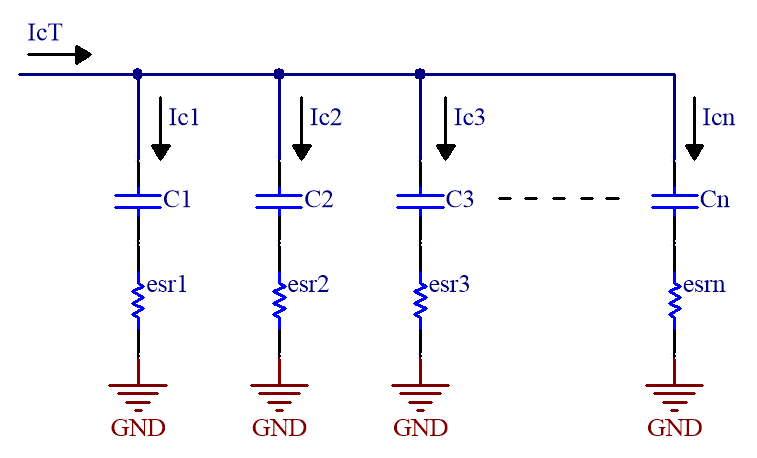
\includegraphics[scale=0.5]{Capacitores-fuente.png}
	\caption{Capacitores de la fuente.}
	\label{fig:img_capacitores-fuente}
\end{figure}


\begin{equation} 
	C = C1 + C2 + ... + C_n
\end{equation}


\noindent Si todos los valores de ESR son iguales se obtiene:

\begin{equation} 
R_T = \frac{R_{ESR}}{n}
\end{equation}

\noindent Por lo tanto, se puede calcular la potencia que disipan como:

\begin{equation}\label{eq_potencia} 
	P = I^2 * R_T = 21.25^2 * \frac{R_{ESR}}{n}
\end{equation}

\noindent Se decidió utilizar 6 capacitores  de $2200 \:uF$ con un rating de tensión de $50\:V$ y una ESR de $17 \:\Omega$ (datos obtenidos de \cite{EKY-350ELL222MM25S}) . De esta forma, al reemplazar en la ecuación \ref{eq_potencia} se obtiene que la potencia disipada es de: 

\begin{equation} 
	P=1.28\:W
\end{equation}


\subsection{Conmutación de alta frecuencia para el \textsl{bootstrap}}
\label{secc_conmutacion-auxiliar}

\noindent Cuando el MOSFET \textsl{driver} recibe una entrada que activa un MOS del lado superior, este comienza a cargar el \textsl{gate} con ayuda de la tensión que brinda el capacitor de \textsl{bootstrap} asociado a ese MOS. El capacitor de \textsl{bootstrap} entrega energía durante la carga del \textsl{gate} y durante todo el tiempo que el MOS esté activo (debido a la resistencia $R_{GS}$). Para poder recargar el capacitor, debe esperarse a que el \textsl{driver} reciba la entrada necesaria para apagar el MOS. Debido a que la implementación del \textsl{driver} de corriente utiliza un controlador por histéresis, no es posible asegurar que haya una conmutación en un periodo regular.

\noindent Para poder asegurar un periodo de conmutación constante y conocido se agrega un bloque que superpone una conmutación de alta frecuencia a la señal de control que ingresa al MOSFET \textsl{driver}. De esta manera se producen conmutaciones en un intervalo regular que permiten la carga de los capacitores de \textsl{bootstrap}. 

\noindent Se adopta una frecuencia de conmutación auxiliar de $50\:kHz$ y se hace variar el ciclo de trabajo de la salida del comparador con histéresis entre dos valores. Para la carga del inductor se definió que el ciclo de trabajo sea del 90\% mientras que para la descarga sea del 10\%.

\noindent Para generar esta conmutación se agrega el oscilador que se observa en la figura \ref{fig:img_frecuencia-auxiliar} a la salida del comparador con histéresis. La frecuencia de conmutación se puede obtener en función de $C_1$ como:

\begin{equation} 
	F_{aux} = \frac{4.5*10^{-5}}{C1} [Hz]
\end{equation}


\noindent Esta frecuencia debe ser mucho mayor a la fundamental de la corriente triangular para evitar problemas en el funcionamiento del sistema y, además, debe ser lo suficientemente alta para poder ser filtrada sin inconvenientes en la etapa de estimación de posición (como se explica en el capítulo \ref{cap:Estimador Analogico}). Por lo tanto, al adoptar una frecuencia auxiliar de $50\:kHz$, resulta en $C_1= 900\:pF$.

\begin{figure}[H]
	\centering
	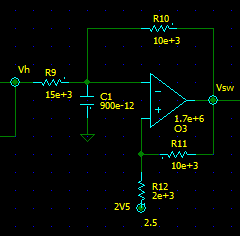
\includegraphics[scale=1]{Frecuencia-auxiliar.png}
	\caption{Circuito oscilador de frecuencia auxiliar.}
	\label{fig:img_frecuencia-auxiliar}
\end{figure}


\subsection{Simulación del sistema con oscilador auxiliar}

\noindent En la figura \ref{fig:img_corriente-auxiliar} se muestran las formas de onda obtenidas con el oscilador auxiliar utilizado para el correcto funcionamiento del \textsl{bootstrap}. 

\begin{figure}[H]
	\centering
	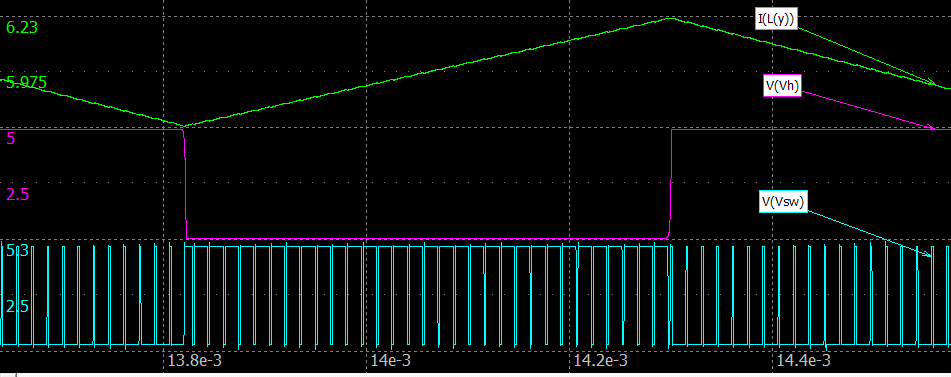
\includegraphics[scale=0.5]{Corriente-auxiliar.png}
	\caption{Simulación de corriente en el electroimán, salida del comparador, y conmutación auxiliar.}
	\label{fig:img_corriente-auxiliar}
\end{figure}

\section{Criterio de utilización de la topología de puente H}
\label{secc_justificación-puente-H}

\noindent Es necesario que el controlador presente una corriente media unidireccional, ya que una corriente media negativa es indistinguible de la positiva puesto que tiene el mismo efecto en la fuerza del electroimán, pero el signo del controlador hace inestable el lazo de control. Sin embargo, puede darse el caso que la corriente en el electroimán sea negativa de manera instantánea con valor medio positivo. En ese caso, es necesario que se conserve la forma de onda triangular ya que de lo contrario traería problemas en la estimación de la posición (como se explica en el capítulo \ref{cap:Estimador Analogico}). Por lo tanto, para evitar que la misma sea recortada, es necesario que el controlador permita excursiones negativas sin perder la forma de onda. Esta situación puede darse en los siguientes casos:


\begin{itemize} 
	\item Cuando el sistema arranca desde corriente cero, hasta que el valor medio de corriente supera la mitad del ripple de corriente $(\Delta I_{L})$.
	
	\item Cuando el entrehierro es pequeño y se trabaja con peso reducido la corriente media puede llegar a ser menor que el ripple $\Delta I_{L}$.
\end{itemize}

\noindent Por estos motivos se debe utilizar una topología de puente completo, puesto que permite la excursión negativa de la corriente mientras que mantiene en funcionamiento al estimador de posición.

\subsection{Ajuste para evitar lazo abierto con corriente instantánea negativa}

\noindent El sensor de efecto Hall entrega una tensión proporcional a la corriente que circula por el electroimán con un \textsl{offset} de $2.5\:V$. Es decir, para corrientes positivas, la salida será mayor a $2.5\:V$, y para corrientes negativas, menor.

\noindent La salida de este sensor se realimenta hacia la entrada del controlador de corriente mediante un operacional, quitándole el \textsl{offset} de $2.5\:V$. Debido a que se utiliza una fuente simple para la alimentación, el circuito encargado de realimentar solo permite excursiones positivas de la corriente mientras que las negativas son recortadas. Esto presenta un problema ya que si ocurre el caso de que la corriente del electroimán se haga negativa instantáneamente, la tensión de salida del sensor de efecto Hall será menor a $2.5\:V$, por lo que la salida del operacional será recortada y, por lo tanto, el sistema quedará a lazo abierto.

\noindent Para solucionar este problema se analizaron dos alternativas:

\begin{itemize} 
	\item Elevar el \textsl{set-point} del sensor de efecto Hall.
	
	\item Utilizar una alimentación bipolar para el operacional de realimentación.
\end{itemize}

\noindent Entre estas se eligió la primer alternativa, ya que se puede implementar con mayor facilidad en el circuito. Hay que tener en cuenta que, al incrementar el \textsl{offset} del sensor, también se debe incrementar en la misma proporción la tensión de referencia de la etapa de entrada al controlador de corriente.

\noindent Para saber qué valor utilizar para el \textsl{offset} se debe calcular el mínimo de tensión entregada por el sensor de efecto Hall. Esto se da cuando la referencia del controlador de corriente es de $0\:V$, con lo cual la corriente media del electroimán será $0 \:A$ con una excursión de $±250\:mA$. Lo que significa una tensión de salida del sensor de efecto Hall de $13.3\:mV$ por encima y debajo del \textsl{offset}. Para tomar un margen se incrementa el \textsl{offset} a $2.6\:V$. 



\section{Características estáticas y dinámicas del controlador}

\subsection{Corriente media del electroimán}

\noindent Para saber la corriente media que hay a la salida al aplicarle cierta tensión en la entrada, se utiliza la transferencia de lazo cerrado (sin considerar polos, y suponiendo alta ganancia de lazo abierto):

\begin{equation} 
	I_L = V_{iLRef} * \frac{K_{in}}{H(s)} = V_{iLRef} * 6 \frac{A}{V}
\end{equation}

\subsection{Frecuencia de conmutación de la corriente}

\noindent La frecuencia de conmutación del sistema se obtiene con:

\begin{equation}\label{eq_frec-sw} 
f_{SW} = \frac{V_{BUS}}{2*\Delta I_L * L(Y_g)}
\end{equation}

\noindent Para $Y_g = 4 \:mm $ se tiene una inductancia $L(4\:mm) = 16.44 \:mHy$ , lo cual resulta en una frecuencia $f_{SW }= 1460 \:Hz$ .

\subsection{Ancho de banda del controlador}\label{esccion_AB_Controlador} 

\noindent La dinámica del controlador, al depender de la inductancia, lo hace también del entrehierro. El ancho de banda (o velocidad con que responde) está limitado por la constante de tiempo del inductor con su resistencia serie. Juntas forman un sistema lineal de primer orden, con un polo en: 

\begin{equation} \label{eq_frec-angular}
	\omega _{polo} = \frac{R_L}{L(Y_g)}
\end{equation}

\noindent Al tomar las condiciones del problema en el punto de linealización con $Y_{0}=4\:mm$, resulta una inductancia $L = 7.55 \:mHy + 8.89 \:mHy$. Luego, al considerar la resistencia del bobinado $R_L=0.2\:\Omega$, se calcula la ubicación del polo:

\begin{equation} 
	\omega _{polo} = \frac{0.2\:\Omega}{16.44 \:mHy} = 12.17 \:rad/s
\end{equation}

\noindent La tabla \ref{tab_mediciones} muestra  entre qué valores de frecuencia se ve afectada la forma de onda al modificarse la distancia de separación.

\begin{equation} \label{eq_DeltaT}
	\Delta T [s] = \frac{\Delta I_L * (L(Y_g) + L_{\infty})}{V_{BUS}}
\end{equation}

\noindent En la ecuación \ref{eq_DeltaT}, $\Delta T$ representa el tiempo de crecimiento o de decrecimiento de la rampa de corriente (sin considerar la resistencia del bobinado) en torno al valor nominal. El doble de este tiempo es igual al periodo de la corriente triangular $(2*T=\frac{1}{F_{SW}})$.

\noindent Según las mediciones de inductancia realizadas y, al aplicar las ecuaciones \ref{eq_frec-sw}, \ref{eq_frec-angular} y \ref{eq_DeltaT}, se obtuvo la tabla \ref{tab_mediciones}.


\begin{table}[H]
	\begin{center}
		\begin{tabular}{| c | c | c | c | c |}
			\hline
			$Y_g\:[mm]$ & $L(Y_g)\:[mHy]$ & $\Delta T\:[ms]$ & $f_{SW}\:[Hz]$ & $\omega _{polo}\:[rad/s]$\\ \hline
			0 & 76.45 & 1.59 & 313.93 & 2.62\\ \hline
			1 & 33.42 & 0.70 & 718.13 & 5.98\\ \hline
			2 & 22.64 &	0.47 & 1060.07 & 8.83\\ \hline
			3 &	18.8 & 0.39 & 1276.60 & 10.64\\ \hline
			4.4 & 15.5 & 0.32 & 1548.39 & 12.90\\ \hline
			5.2 & 14.7 & 0.31 & 1632.65 & 13.61\\ \hline
			6.5 & 14.4 & 0.30 & 1666.67 & 13.89\\ \hline
			8.23 & 12.4 & 0.26 & 1935.48 & 16.13\\ \hline
			$\infty$ & 8.89 & 0.19 & 2699.66 & 22.5	\\ \hline
		\end{tabular}
		\caption{Valores calculados y medidos en función del entrehierro.}
		\label{tab_mediciones}
	\end{center}
\end{table}

\subsection{Transferencia lineal del controlador de corriente}

\noindent En la ecuación \ref{eq_TLC-cc} se muestra la transferencia linealizada del controlador de corriente para una distancia de separación de $Y_{0}=4\:mm$.

\begin{equation} \label{eq_TLC-cc}
G_{iL}(s) = \frac{6}{1+\frac{s}{12.17}}
\end{equation}

